\documentclass[a4paper, 12pt]{article}
\usepackage{geometry}
\geometry{a4paper,
total={170mm,257mm},left=2cm,right=2cm,
top=2cm,bottom=2cm}

\usepackage{mathtext}
\usepackage{amsmath}
\usepackage[T2A]{fontenc}
\usepackage[utf8]{inputenc}
\usepackage[english,russian]{babel}
\usepackage{graphicx, float}
\usepackage{tabularx, colortbl}
\usepackage{caption}
\captionsetup{labelsep=period}

\newcommand{\parag}[1]{\paragraph*{#1:}}
\DeclareSymbolFont{T2Aletters}{T2A}{cmr}{m}{it}
\newcounter{Points}
\setcounter{Points}{1}
\newcommand{\point}{\arabic{Points}. \addtocounter{Points}{1}}
\newcolumntype{C}{>{\centering\arraybackslash}X}

\author{Калинин Даниил, Б01-110}
\date{\today}
\title{Лабораторная работа 2.1.6. Эффект Джоуля-Томпсона}

\begin{document}
\maketitle

\parag {Цель работы}
\begin{enumerate}
    \item  определение изменения температуры углекислого газа при протекании через малопроницаемую перегородку при разных начальных значениях давления и температуры;
    \item вычисление по результатам опытов коэффициентов Ван-дер-Ваальса «a» и «b».
\end{enumerate}

\parag {В работе используются}
трубка с пористой перегородкой; труба Дьюара; термостат; термометры; дифференциальная термопара; микровольтметр; балластный баллон; манометр.

\parag {Экспериментальная установка}~\\
\begin{figure}[H]
    \centering
    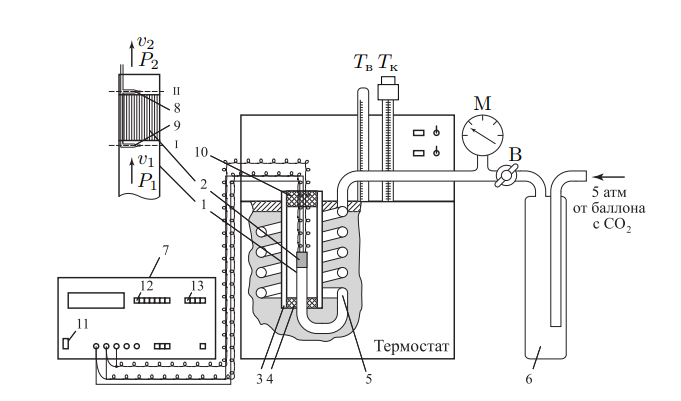
\includegraphics[width=\linewidth]{setup.png}
    \caption{\textit{Установка, на которой проводился эксперимент}}
    \label{setup}
\end{figure}

\parag {Теоритическая справка} ~\\
Эффектом  Джоуля–Томсона называется изменение температуры газа, медленно протекающего из области высокого в область низкого давления в условиях хорошей тепловой изоляции.

Рассмотрим стационарный поток газа между произвольными сечениями I и II трубки (до перегородки и после неё). Пусть, для определённости, через трубку прошёл 1 моль углекислого газа; $\mu$ — его молярная масса. Молярные объёмы газа, его давления и отнесённые к молю внутренние энергии газа в сечениях I и II обозначим соответственно $V_1$, $P_1$, $U_1$ и $V_2$, $P_2$, $U_2$. Для того чтобы ввести в трубку объём $V_1$, над газом нужно совершить работу $A_1 = P_1 V_1$. Проходя через сечение II, газ сам совершает работу $A_2 = P_2 V_2$. Так как через боковые стенки не происходит ни обмена теплом, ни передачи механической энергии, то

\begin{equation}
    A_1 - A_2 = \left(U_2 - \frac{\mu v_2^2}{2}\right) - \left(U_1 -  \frac{\mu v_1^2}{2}\right)
    \label{eq:1}
\end{equation}

В уравнении \eqref{eq:1} учтено изменение как внутренней (первые члены в скобках), так и кинетической (вторые члены в скобках) энергии газа. Подставляя в \eqref{eq:1} написанные выражения для $A_1$ и $A_2$ и перегруппировывая члены, найдём:

\begin{equation}
    H_1 - H_2 = \left(U_1 + P_1V_1\right) - \left(U_2 + P_2V_2\right) =  \frac{1}{2}\mu\left(v_2^2 - v_1^2\right)
    \label{eq:2}
\end{equation}

\begin{equation}
    \mu_{д-т} = \frac{\Delta T}{\Delta P} \approx \frac{\frac{2a}{RT} - b}{C_P}
    \label{eq:3}
\end{equation}

Из формулы \eqref{eq:3} видно, что эффект Джоуля–Томсона для не очень плотного газа зависит от соотношения величин a и b, которые оказывают противоположное влияние на знак эффекта. Если силы взаимодействия между молекулами велики, так что превалирует «поправка на давление», то основную роль играет член, содержащий a, и

\begin{equation*}
    \frac{\Delta T}{\Delta P} > 0
\end{equation*}

т. е. газ при расширении охлаждается ($\Delta T < 0$, так как всегда $\Delta P < 0$). В обратном случае (малые a)

\begin{equation*}
    \frac{\Delta T}{\Delta P} < 0
\end{equation*}

т.е. газ нагревается ($\Delta T > 0$, так как по-прежнему $\Delta P < 0$)

\begin{equation}
    T_{инв} = \frac{27}{4}T_{кр.}
\end{equation}

При температуре $T_{инв}$ эффект Джоуля–Томсона меняет знак: ниже температуры инверсии эффект положителен ($\mu_{д-т} > 0$, газ охлаждается), выше $T_{инв}$ эффект отрицателен ($\mu_{д-т} < 0$, газ нагревается).

Заменяя в формуле \eqref{eq:2} $U$ через $C_V$, $T$ и $PV$ через $RT$ , найдём:

\begin{gather*}
    \left(R + C_v\right)\left(T_1 - T_2\right) = \mu \frac{\left(v_2^2 - v_1^2\right)}{2}, \\
    \Delta T = \frac{\mu}{2 C_p}\left(v_2^2 - v_1^2\right)
\end{gather*}

В условиях нашего опыта расход газа $Q$ на выходе из пористой перегородки не превышает 10 $см^3/с$, а диаметр трубки равен 3 мм. Поэтому

\begin{equation*}
    u_2 \leq \frac{4Q}{\pi d^2} = \frac{4 \cdot 10~см^3/с}{3.14 \cdot (0.3)^2~см^2} \approx 140~см/с 
\end{equation*}

Скорость $v_1$ газа у входа в пробку относится к скорости $v_2$ у выхода из неё как давление $P_2$ относится к давлению $P_1$. В нашей установке $P_1$ = 4 атм, a $P_2$ = 1 атм, поэтому

\begin{equation*}
    u_1 = \frac{P_2}{P_1}v_2 = \frac{1~атм}{4~атм} \cdot 140~см/с = 35~см/с 
\end{equation*}

\begin{equation*}
    \Delta T = \frac{\mu}{2C_p}\left(v_2^2 - v_1^2\right) = \frac{44 \cdot 10^{-3}}{2 \cdot 40}\left(1.4^2 - 0.35^2\right) = 7\cdot10^{-4}~K
\end{equation*}

Это изменение температуры ничтожно мало по сравнению с измеряемым эффектом (несколько градусов).


\parag {Ход работы} ~\\
\point Для начала запишем погрешности:
\begin{enumerate}
    \item $\sigma_p = 0.05~атм.$
    \item $\sigma_U = 0.5~мкВ.$
\end{enumerate}

\point Включаем термостат, устанавливаем температуру $22.8^\circС$. Открываем вентиль так, чтобы избыточное давление было примерно 4 атм., ждём установления равновесия (1.5-2 минуты) записываем показания вольтметра в таблицу, далее проделываем аналогичные операции при избыточном давлении примерно 3.4, 3, 2.5, 2, результаты записываем в таблицу. Далее полученные значения напряжения переводим в значения температуры согласно таблице, указанной в описании работы.

\point Строим график зависимости $\Delta P (\Delta P)$, при помощи МНК находим коэффициент угла наклона графика, рассчитываем погрешность полученного значения. Проделываем действия пп.1-2 для температур в диапазоне 20-60 $^\circС$ с интервалом 10-20 $^\circС$. Результаты занесем в таблицы \ref{tabl:data_22.8}, \ref{tabl:data_30} и \ref{tabl:data_50}.

\begin{table}[h]
    \centering
    \begin{tabular}{|c|c|c|}\hline
    \multicolumn{3}{|c|}{$T = 22.8^\circ C$}\\ \hline
    $\Delta P$, атм.	& Напряжение, мкВ.	& $\Delta T,~^\circ C$	\\ \hline
    4	& -164.00	& -3.79	\\ \hline
    3.4	& -140.00	& -3.23	\\ \hline
    3	& -114.00	& -2.63	\\ \hline
    2.5	& -91.00	& -2.10	\\ \hline
    2	& -68.00	& -1.57	\\ \hline
    \end{tabular}
    \caption{Изменение температуры при различных давлениях, при начальной температуре $T = 22.8^\circ C$}
    \label{tabl:data_22.8}
    \end{table}
    
    
    \begin{table}[h]
    \centering
    \begin{tabular}{|c|c|c|}\hline
    \multicolumn{3}{|c|}{$T = 30^\circ C$}\\ \hline
    $\Delta P$, атм.	& Напряжение, мкВ.	& $\Delta T,~^\circ C$	\\ \hline
    4	& -162.00	& -3.98	\\ \hline
    3.4	& -135.00	& -3.32	\\ \hline
    3	& -110.00	& -2.70	\\ \hline
    2.5	& -88.00	& -2.16	\\ \hline
    2	& -64.00	& -1.57	\\ \hline
    \end{tabular}
    \caption{Изменение температуры при различных давлениях, при начальной температуре $T = 30^\circ C$}
    \label{tabl:data_30}
    \end{table}
    
    
    \begin{table}[h]
    \centering
    \begin{tabular}{|c|c|c|}\hline
    \multicolumn{3}{|c|}{$T = 50^\circ C$}\\ \hline
    $\Delta P$, атм.	& Напряжение, мкВ.	& $\Delta T,~^\circ C$	\\ \hline
    4	& -166.00	& -3.99	\\ \hline
    3.4	& -136.00	& -3.27	\\ \hline
    3	& -106.00	& -2.55	\\ \hline
    2.5	& -82.00	& -1.97	\\ \hline
    2	& -58.00	& -1.39	\\ \hline
    \end{tabular}
    \caption{Изменение температуры при различных давлениях, при начальной температуре $T = 50^\circ C$}
    \label{tabl:data_50}
    \end{table}

\point По полученным данным построим графики зависимости $\Delta T \left(\Delta P\right)$. Графики изображены на рисунках \ref{fig:plot_dt_from_dp_T_22.8}, \ref{fig:plot_dt_from_dp_T_30} и \ref{fig:plot_dt_from_dp_T_50}.

\begin{figure}[h]
    \centering
    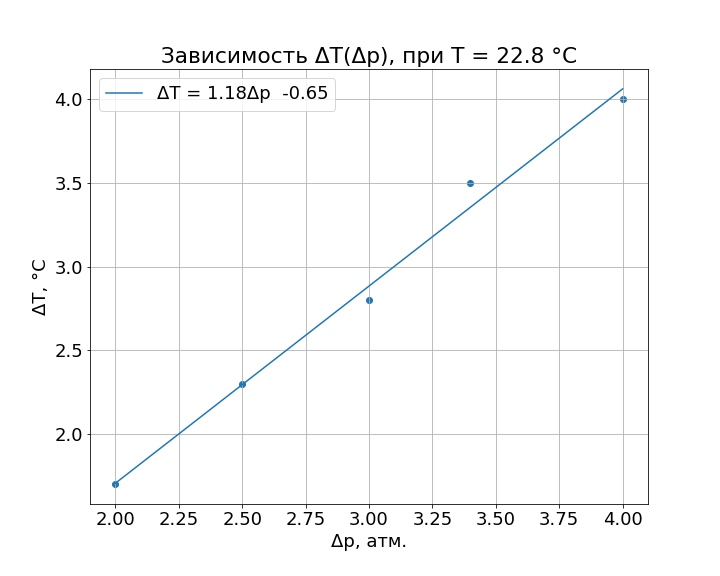
\includegraphics[width=\linewidth]{plot_dt_from_dp_T_22.8.png}
    \caption{\textit{График зависимости $\Delta T \left(\Delta P\right)$ для температуры $T = 22.8 ^\circ C$.}}
    \label{fig:plot_dt_from_dp_T_22.8}
\end{figure}

\begin{figure}[h]
    \centering
    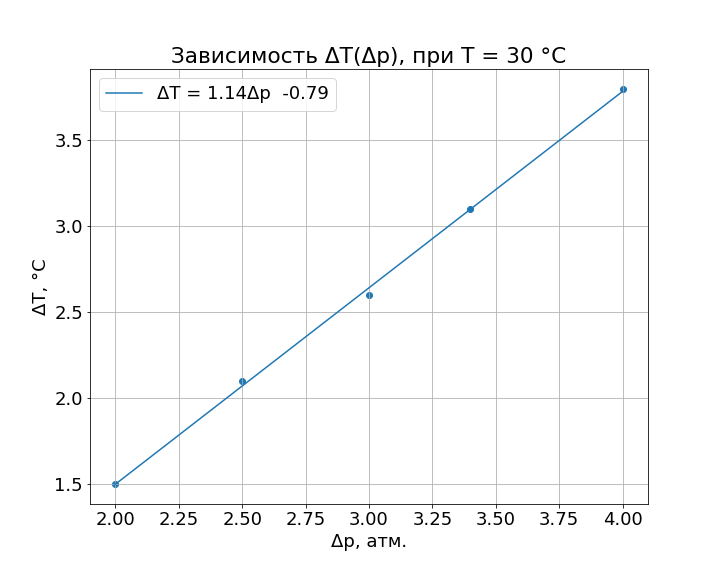
\includegraphics[width=\linewidth]{plot_dt_from_dp_T_30.png}
    \caption{\textit{График зависимости $\Delta T \left(\Delta P\right)$ для температуры $T = 30 ^\circ C$.}}
    \label{fig:plot_dt_from_dp_T_30}
\end{figure}

\begin{figure}[h]
    \centering
    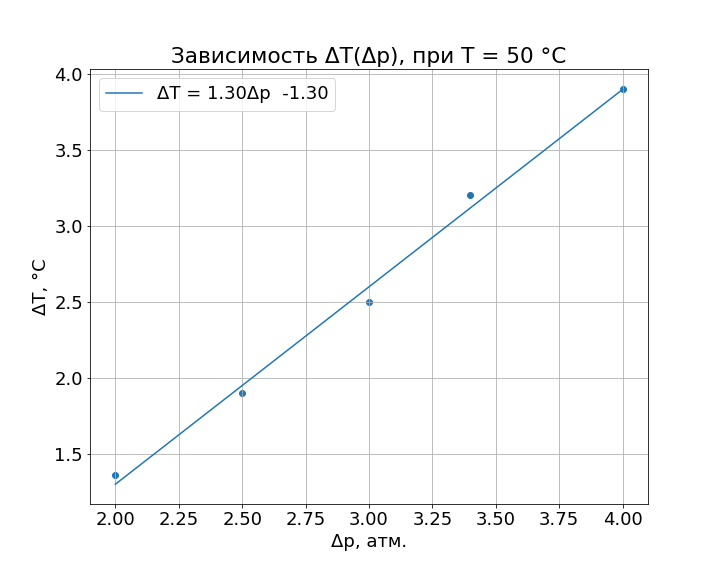
\includegraphics[width=\linewidth]{plot_dt_from_dp_T_50.png}
    \caption{\textit{График зависимости $\Delta T \left(\Delta P\right)$ для температуры $T = 30 ^\circ C$.}}
    \label{fig:plot_dt_from_dp_T_50}
\end{figure}

\point По углу наклона графиков расчитаем коэффициент  $\mu_{д-т}$ и погрешность его вычисления для каждой температуры, воспользовавшись формулами:

\begin{gather*}
    \mu_{д-т} = \frac{d\left(\Delta P\right)}{d\left(\Delta T\right)} \\
    \varepsilon_{mu} = \sqrt{\varepsilon_u^2 + \varepsilon_{P}^2}
\end{gather*}

Результаты занесем в таблицу \ref{tabl:mus}.

\begin{table}[h]
    \centering
    \begin{tabular}{|c|c|c|}\hline
    $T,~^\circ C$.	& $\mu$, К/атм.	& $\varepsilon_{mu},~\%$	\\ \hline
    $22.8$	& $-1.13$	& $1.73$\\ \hline
    $30$	& $-1.22$	& $1.74$\\ \hline
    $50$	& $-1.32$	& $1.74$\\ \hline
    \end{tabular}
    \caption{коэффициент $\mu_{д-т}$ для разных температур}
    \label{tabl:mus}
\end{table}

\point Теперь построим график $\mu\left(1 / T \right)$. Восстановим прямую, воспользовавшись методом МНК. График изобразим на рисунке \ref{fig:mu_from_one_over_T}

\begin{figure}[h]
    \centering
    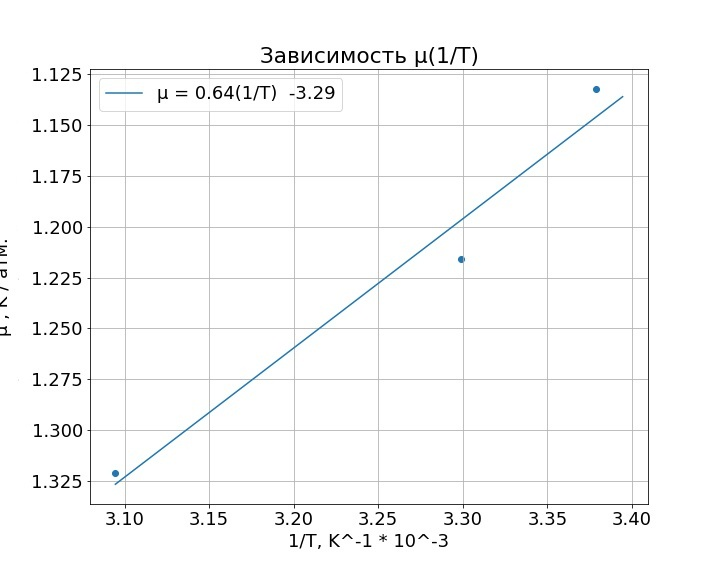
\includegraphics[width=\linewidth]{plot_mu_from_one_over_T.png}
    \caption{График зависимости $\mu\left(1 / T \right)$.}
    \label{fig:mu_from_one_over_T}
\end{figure}

\point Воспользовавшись следующими формулами, рассчитаем коэффициенты в уравнении Ван-дер-Ваальса для исследуемого газа.

\begin{gather*}
    a = \frac{d \left(\mu_{д-т}\right)}{d \left(1 / T\right)} C_p \frac{R}{2} = 0.95~\frac{Н \cdot м^4}{моль^2} \\
    b = -B C_p = 1186~\frac{см^3}{моль}\\
    \varepsilon_{a} = \sqrt{\varepsilon_{\mu}^2 + \varepsilon_{T}^2} = 7\% \\
    \varepsilon_{b} = \varepsilon_{B} \overset{из~МНК}{=} 2.5\%
\end{gather*}


\parag {Заключение} ~\\
В ходе работы были получены коэффициенты Джоуля-Томпсона при различных температурах, также была получена зависимость коэффициента Джоуля-Томпсона от температуры.

Были рассчитаны коэффициенты Ван-дер-Вальса для исследуемого газа. Отметим, что полученные значения не совпадают с табличными даже с учётом погрешности, что говорит о неприменимости в данных условиях модели газа Ван-дер-Вальса.

\end{document}
